\documentclass[a4paper,12pt]{article} % тип документа

% Поля страниц
\usepackage[left=2.5cm,right=2.5cm,
    top=2cm,bottom=2cm,bindingoffset=0cm]{geometry}
    
%Пакет дял таблиц   
\usepackage{multirow} 
    
%Отступ после заголовка    
\usepackage{indentfirst}


% Рисунки
\usepackage{floatrow,graphicx,calc}
\usepackage{wrapfig}

%%% Работа с картинками
\usepackage{graphicx}  % Для вставки рисунков
\graphicspath{{images/}}  % папки с картинками
\setlength\fboxsep{3pt} % Отступ рамки \fbox{} от рисунка
\setlength\fboxrule{1pt} % Толщина линий рамки \fbox{}
\usepackage{wrapfig} % Обтекание рисунков и таблиц текстом

% Создаём новый разделитель
\DeclareFloatSeparators{mysep}{\hspace{1cm}}

% Ссылки?
\usepackage{hyperref}
\usepackage[rgb]{xcolor}
\hypersetup{				% Гиперссылки
    colorlinks=true,       	% false: ссылки в рамках
	urlcolor=blue          % на URL
}


%  Русский язык
\usepackage[T2A]{fontenc}			% кодировка
\usepackage[utf8]{inputenc}			% кодировка исходного текста
\usepackage[english,russian]{babel}	% локализация и переносы

% Математика
\usepackage{amsmath,amsfonts,amssymb,amsthm,mathtools}

%%% Дополнительная работа с математикой
\usepackage{amsmath,amsfonts,amssymb,amsthm,mathtools} % AMS
\usepackage{icomma} % "Умная" запятая: $0,2$ --- число, $0, 2$ --- перечисление

% Что-то 
\usepackage{wasysym}


\begin{document}
\begin{center}
	\footnotesize{ФЕДЕРАЛЬНОЕ ГОСУДАРСТВЕННОЕ АВТОНОМНОЕ ОБРАЗОВАТЕЛЬНОЕ 			УЧРЕЖДЕНИЕ ВЫСШЕГО ОБРАЗОВАНИЯ}\\
	\footnotesize{МОСКОВСКИЙ ФИЗИКО-ТЕХНИЧЕСКИЙ ИНСТИТУТ\\(НАЦИОНАЛЬНЫЙ 			ИССЛЕДОВАТЕЛЬСКИЙ УНИВЕРСИТЕТ)}\\
	\footnotesize{ФИЗТЕХ-ШКОЛА ФИЗИКИ И ИССЛЕДОВАНИЙ им. ЛАНДАУ\\}
	\hfill \break
	\hfill \break
	\hfill \break
	\hfill \break
\end{center}

\begin{center}   
    \hfill \break
	\hfill \break
	\hfill \break
	\hfill \break    \hfill \break
	\hfill \break
	\hfill \break
	\hfill \break
    \hfill \break
    \hfill \break
	\hfill \break
	\large{Лабораторная работа № 2.5.1 \\\textbf{Измерение коэффициента поверхностного натяжения
  жидкости}}\\
	\begin{flushright}
		Плотникова Анастасия Александровна\\
		Группа Б02-406
	\end{flushright}
	\hfill \break
	\hfill \break
	\hfill \break
\end{center}
\hfill \break
\hfill \break
\hfill \break
\hfill \break
\hfill \break
\hfill \break
\hfill \break
\hfill \break
\hfill \break
\hfill \break
\hfill \break
\hfill \break
\hfill \break
\begin{center}
	Долгопрудный, 2025 г.
\end{center}
\thispagestyle{empty}
\newpage
	\textbf{Цель работы:}\\ 
  1) измерение коэффициента поверхностного натяжения исследуемой жидкости при разной температуре с использованием известного коэффициента поверхностного натяжения другой жидкости; \\
  2) определение полной поверхностной энергии и теплоты, необходимой для изотермического образования единицы поверхности жидкости.
	\hfill \break
	
	\textbf{В работе используются:}\\ 
  прибор Ребиндера с термостатом; \\
  исследуемые жидкости; \\
  стаканы.
	
\section*{Теоретическая справка}

Наличие поверхностного слоя приводит к различию давлений по разные стороны от искривленной границы раздела двух сред. Для сферического пузырька с воздухом  внутри жидкости избыточное давление даётся формулой Лапласа:
	\begin{equation}
		\label{laplas}
		\Delta P = \frac{2\sigma}{r},
	\end{equation}
	где $\sigma$ –- коэффициент поверхностного натяжения, $\Delta P$ – разница давлений внутри и снаружи пузырька, $r$ – радиус кривизны поверхности раздела двух фаз. Эта формула лежит в основе предлагаемого метода определения коэффициента поверхностного натяжения жидкости.

\section*{Экспериментальная установка} 

Схема установки изображена на рисунке (\ref{fig:setup}). 

Исследуемая жидкость (дистиллированная вода) наливается в сосуд (колбу) \textbf{В}. Тестовая жидкость  (этиловый спирт) наливается  в сосуд \textbf{E}. При измерениях  колбы герметично закрываются  пробками.   Через одну из двух пробок  проходит полая металлическая игла \textbf{C}. Этой пробкой закрывается сосуд, в котором  проводятся измерения. Верхний конец иглы открыт в атмосферу, а нижний погружен в жидкость. Другой сосуд герметично закрывается второй пробкой. При создании достаточного  разряжения воздуха в колбе с иглой пузырьки воздуха начинают пробулькивать через жидкость. Поверхностное натяжение можно определить по величине разряжения $\Delta P$ (\ref{laplas}), необходимого для прохождения пузырьков (при известном радиусе иглы).
	
Разряжение в системе создается с помощью аспиратора \textbf{A}. Кран \textbf{K2} разделяет две полости аспиратора. Верхняя полость при закрытом кране \textbf{K2}  заполняется водой. Затем кран \textbf{K2} открывают и заполняют водой  нижнюю полость  аспиратора.  Разряжение воздуха создается в нижней полости  при открывании крана \textbf{K1}, когда  вода вытекает из неё по каплям. В колбах \textbf{B} и \textbf{C}, соединённых трубками с нижней полостью аспиратора,  создается такое же пониженное давление. Разность давлений в полостях с разряженным воздухом и атмосферой измеряется спиртовым микроманометром.

	\begin{figure}[h!]
		\centering
    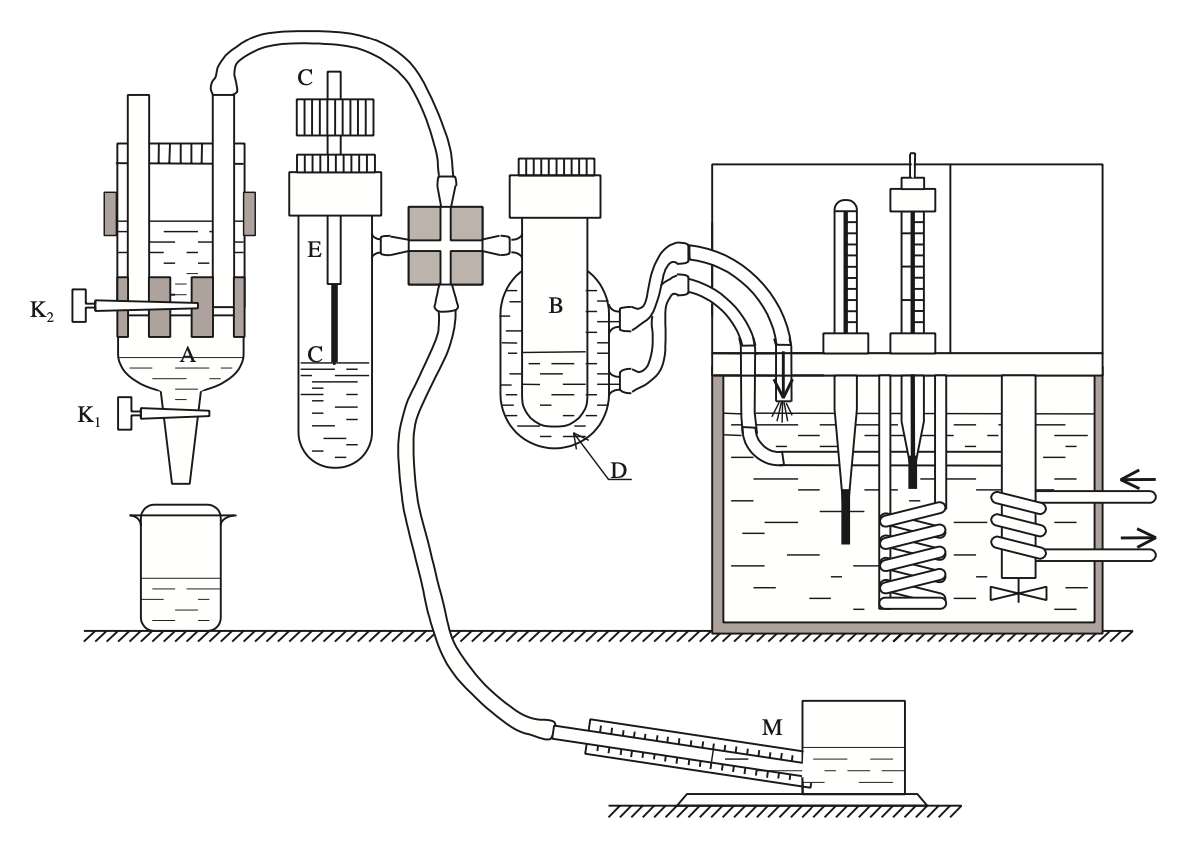
\includegraphics[scale = 0.75]{setup.png}
		\caption{Схема установки для измерения температурной зависимости коэффициента поверхностного натяжения.}
		\label{fig:setup}
	\end{figure}

\section*{Ход работы}

\begin{enumerate}
  \item Убедимся в исправности установки. Для этого заполним аспиратор водой и убедимся, что игла не испачкана анилином (в противном случае промоем её сначала ацетоном, а затем дистиллированной водой), и установим иглу в сосуде с водой так, чтобы её кончик лишь коснулся поверхности воды. Установив скорость падения капель примерно 1 капля в 5 секунд, добьёмся пробулькивания пузырьков. Манометр должен показать медленный рост давления до некоторого максимального значения и затем быстрое его падение при пробулькивании пузырька.
  
  \item Подберём частоту падения капель так, чтобы максимальное давление не зависело от этой частоты. Для этого пузырьки не должны пробулькивать слишком часто (не чаще, чем 1 пузырёк в 5 секунд).
  
  \item Измерим максимальное давление при пробулькивании пузырька. По разбросу результатов оценим случайную погрешность. Пользуясь табличным значением коэффициента поверхностного натяжения воды, определим диаметр иглы. Сравним полученный результат с прямыми измерениями диаметра иглы.
  
  \item Перенесём иглу в сосуд с анилином. Измерим максимальное давление в пузырьках, когда игла лишь касается поверхности жидкости. Измерим $h_1$.
  
  \item Утопим иглу до предела (между концом иглы и дном необходимо оставить небольшой зазор, чтобы образующийся пузырёк не касался дна). Измерим максимальное давление в пузырьках. По разности давлений в этом и предыдущем пункте определим глубину погружения. Измерим $h_2$. Сравним измеренное $\Delta h = h_1 - h_2$ с рассчитанным по $\Delta P$.
  
  \item Проведём измерения при комнатной температуре. Затем снимем зависимость $\sigma(T)$ при нагревании анилина. Для этого включим термостат и подождём, пока нужная температура стабилизируется. Измерения будем проводить через 3--5 градусов, так как нагревать выше 60~$^{\circ}$C не следует, а получиться должно 6--8 точек. Кнопку «Pump» не выключим!
  
  \item Повторим измерения, понижая температуру до комнатной. Для охлаждения через термостат пропустим водопроводную воду.
  
  \item Оценим погрешности измерения давления и температуры.
  
  \item Построим график $\sigma$ от $T$ и с его помощью определим $d\sigma/dT$. Оценим точность результата.
  
  % \item На том же графике изобразим зависимость от температуры теплоты образования единицы площади поверхности $q$ (5.10) и поверхностной энергии единицы площади поверхности $U_п/\Pi$ (5.9).
\end{enumerate}


\begin{table}[h]
  \caption{}
  \begin{tabular}{|c|c|c|}
      \hline $T$, $^\circ C$  &  $\Delta h$, мм & $P$, Па \\
      \hline  &  &  \\
      \hline  &  &  \\
      \hline  &  &  \\
      \hline  &  &  \\
      \hline  &  &  \\
      \hline  &  &  \\
      \hline  &  &  \\
      \hline  &  &  \\
      \hline  &  &  \\
      \hline  &  &  \\
      \hline 
  \end{tabular}
  \label{tab:}
\end{table}

\section*{Вывод}
\end{document}
